\documentclass[11pt,fleqn]{article}
\usepackage[margin=1in,top=1in,bottom=1in]{geometry}
\usepackage{tikz}
\usepackage{mathtools}
\usepackage{longtable}
\usepackage{enumitem}
\usepackage{hyperref}
%\usepackage[dvips]{graphics}
%\usepackage[table]{xcolor}
%\usepackage{amssymb}
\usepackage{float}
%\usepackage{subfig}
\usepackage{booktabs}
\usepackage{subcaption}

\usepackage[normalem]{ulem}

\usepackage{multicol}
\usepackage{txfonts}
\usepackage{amsfonts}
\usepackage{natbib}
\usepackage{gb4e}
\usepackage[all]{xy}
\usepackage{rotating}
\usepackage{tipa}
\usepackage{multirow}
\usepackage{authblk}
\usepackage{url}
\usepackage{pdflscape}
\usepackage{rotating}
\usepackage{adjustbox}
\usepackage{array}

\def\bad{{\leavevmode\llap{*}}}
\def\marginal{{\leavevmode\llap{?}}}
\def\verymarginal{{\leavevmode\llap{??}}}
\def\swmarginal{{\leavevmode\llap{4}}}
\def\infelic{{\leavevmode\llap{\#}}}

\definecolor{airforceblue}{rgb}{0.36, 0.54, 0.66}
%\definecolor{gray}{rgb}{0.36, 0.54, 0.66}

\newcommand{\dashrule}[1][black]{%
  \color{#1}\rule[\dimexpr.5ex-.2pt]{4pt}{.4pt}\xleaders\hbox{\rule{4pt}{0pt}\rule[\dimexpr.5ex-.2pt]{4pt}{.4pt}}\hfill\kern0pt%
}

\setlength{\parindent}{.3in}
\setlength{\parskip}{0ex}

\newcommand{\yi}{\'{\symbol{16}}}
\newcommand{\nasi}{\~{\symbol{16}}}
\newcommand{\hina}{h\nasi na}
\newcommand{\ina}{\nasi na}

\newcommand{\foc}{$_{\mbox{\small F}}$}

\hyphenation{par-ti-ci-pa-tion}

\setlength{\bibhang}{0.5in}
\setlength{\bibsep}{0mm}
\bibpunct[:]{(}{)}{,}{a}{}{,}

\newcommand{\6}{\mbox{$[\hspace*{-.6mm}[$}} 
\newcommand{\9}{\mbox{$]\hspace*{-.6mm}]$}}
\newcommand{\sem}[2]{\6#1\9$^{#2}$}
\renewcommand{\ni}{\~{\i}}

\newcommand{\citepos}[1]{\citeauthor{#1}'s \citeyear{#1}}
\newcommand{\citeposs}[1]{\citeauthor{#1}'s}
\newcommand{\citetpos}[1]{\citeauthor{#1}'s (\citeyear{#1})}

\newcolumntype{R}[2]{%
    >{\adjustbox{angle=#1,lap=\width-(#2)}\bgroup}%
    l%
    <{\egroup}%
}
\newcommand*\rot{\multicolumn{1}{R{90}{0em}}}% no optional argument here, please!


\title{Higher-probability content is more projective than lower-probability content}

%\thanks{For helpful comments on the research presented here, we thank the audience at the 2018 Annual Meeting of XPRAG.de and at the University of T\"ubingen. We gratefully acknowledge financial support for this research from {\em National Science Foundation} grant BCS-1452674 (JT) and the Targeted Investment for Excellence Initiative at The Ohio State University (JT). IGOR Tuebingen}}

\author{Author(s)}

%\author[$\bullet$]{Judith Degen}
%\author[$\circ$]{Judith Tonhauser}

%\affil[$\bullet$]{Stanford University}
%\affil[$\circ$]{The Ohio State University / University of Stuttgart}

\renewcommand\Authands{ and }

\newcommand{\jt}[1]{\textbf{\color{blue}JT: #1}}

\begin{document}

%\tableofcontents
%\newpage

\maketitle

\vspace*{-1cm}

\begin{abstract}

abstract

\end{abstract}

			
\section{Introduction}\label{s1}

A hallmark of the content of the complement (CC) of factive predicates like {\em know}  is that it projects. For example, in an utterance of the sentence \emph{Does Jane know that Sam has a new hat}, the speaker is typically taken to be committed to Sam having a new hat, despite the predicate and the CC being embedded under an entailment-canceling operator (the polar interrogative). The same is typically not true when replacing \emph{know} with a non-factive predicate like \emph{think}. However,  \citealt*{tbd-variability} ({\em Journal of Semantics}) recently showed that there is substantial variability in the projectivity of CCs. While a lot of this variability was explained by the not-at-issueness of the CC, they also found that the lexical content of the CC played a role: e.g., the CC \emph{Sam has a new BMW} was less likely to project than \emph{Sam has a new hat}. The authors hypothesized that the projectivity of a CC may depend on its prior subjective probability, such that a CC is more projective the higher its prior probability. The current work finds support for this hypothesis in an experimental investigation of CCs of both factive and non-factive predicates in which the prior probability of the CC was systematically manipulated. We argue that this finding provides support for constraint-based projection analyses that derive the projectivity of utterance content from the integration of multiple cues, including prior CC probability and the meanings of clause-embedding predicates.

\footnote{\label{f-github}The experiments, data and R code for generating the figures and analyses of the experiments reported on in this paper are available at [redacted for review].}
%\url{https://github.com/judith-tonhauser/factivity}.}  

The 20 predicates we investigated are listed in (\ref{pred}) with the categories they are typically taken to fall into: factive predicates in (\ref{pred}a), non-factive predicates in (\ref{pred}b) and optionally factive predicates in (\ref{pred}c). Specifically, the 5 factive predicates in (\ref{pred}a) include the cognitive predicate {\em know}, the change-of-states predicates {\em discover} and {\em reveal}, the sensory predicate {\em see}, and the emotive predicate {\em be annoyed}. The 6 non-factive predicates in (\ref{pred}b) include 4 `non-veridical non-factive' predicates {\em pretend, suggest, say} and {\em think}, whose CC is typically taken to be neither presupposed nor entailed, as well as  2 `veridical non-factive' predicates {\em be right} and {\em demonstrate}, whose CC is typically taken to be entailed but not presupposed.\footnote{\citet{anand-hacquard2014} assumed that {\em demonstrate} is veridical, in contrast to \citealt{anand-etal2019}. This latter work also takes {\em reveal} to be non-factive, in contrast to, for instance, \citealt{egre2008,wyse} or \citealt{tbd-variability}.}  The 9 optionally factive predicates in (\ref{pred}c) include {\em acknowledge, admit} and {\em announce}, which \citealt{kiparsky-kiparsky70} listed as optionally factive, as well as {\em confirm, inform, confess, establish, hear} and {\em prove}.\footnote{Different categories have been assumed for these 6 predicates. For {\em confirm} and {\em inform}, \citet{anand-hacquard2014} took them to be optionally factive, but recall from above that \citet{schlenker10} took {\em inform} to be factive. For {\em prove}, \citet{white-rawlins-nels2018} suggested that it is optionally factive, but \citet{anand-hacquard2014} took it to be non-veridical and non-factive. For {\em confess}, \citet{swanson2012} took it to be factive, \citet{karttunen2016} only took it to commit the speaker to the subject of the attitude being committed to the CC, and \citet{wyse} listed it under the non-factive predicates. For {\em establish}, \citet{swanson2012} took it to be non-factive, but \citet{wyse} listed it under the factive predicates. Finally, we also included {\em hear} in this class: even though it is often considered a factive sensory predicate (e.g., \citealt{beaver-belly,anand-hacquard2014}), it has been observed that {\em hear} also has a non-factive reportative evidential sense (see, e.g., \citealt{anderson86,simons07}), especially when it is combined with complements that describe events that cannot be auditorily perceived, as is the case in our experiments.}

\begin{exe}
\ex\label{pred} 20 clause-embedding predicates 

\begin{xlist}

\ex factive: {\em be annoyed, discover, know, reveal, see}

\ex non-factive:

\begin{xlist}

\ex non-veridical non-factive: {\em pretend, suggest, say, think}

\ex veridical non-factive: {\em be right, demonstrate}

\end{xlist}

\ex optionally factive: {\em acknowledge, admit, announce, confess, confirm, establish, hear, inform, prove}

\end{xlist}

\end{exe}

\section{Methods}\label{s2}

Exp.~1 was designed to explore projectivity of the CC of the 20 clause-embedding predicates. It used the `certain that' diagnostic for projectivity (see also, e.g., \citealt{tonhauser-salt26,djaerv-bacovcin-salt27,stevens-etal2017,tbd-variability,mahler-nels,demarneffe-etal-sub23}): on this diagnostic, participants are presented with an utterance in which the content to be investigated occurs in an entailment-canceling environment, like a polar question, as illustrated in (\ref{stim}) for the content of the nominal appositive, that Martha's new car is a BMW.

\begin{exe}

\ex\label{stim} Patrick asks: {\em Was Martha's new car, a BMW, expensive?} 

\end{exe}
To assess projectivity, that is, whether the speaker presupposes the truth of the content, participants are asked whether the speaker is certain of the content; for instance, in (\ref{stim}), participants are asked whether Patrick is certain that Martha's new car is a BMW. If a listener takes the speaker to be certain of the content, we assume that the content projects, that is, the speaker presupposes its truth; if a listener does not take the speaker to be certain of the content, we assume that the content does not project, that is the speaker does not presuppose its truth.

Following \citealt{tbd-variability}, Exp.~1 implemented the `certain that' diagnostic with a gradient response scale: participants gave their responses on a slider marked `no' at one end (coded as 0) and `yes' at the other (coded as 1). We assume that the higher a participant's response is, the more the participant takes the speaker to be certain of the content, that is, the more projective the content is. As discussed in \citealt{tbd-variability}, at least two interpretations are compatible with gradient certainty ratings: on a first interpretation, a listener's gradient certainty ratings indicates gradience in the speaker's commitment to the truth of the content; on a second, speaker commitment to the truth of utterance content is binary and categorical, and a listener's gradient certainty rating indicates the listener's degree of belief in the speaker's commitment the truth of the content. We remain agnostic here about the interpretation of gradient certainty ratings:  according to the first definition of factive predicates, either interpretation gives rise to the expectation that certainty ratings for factive predicates are categorically higher than for optionally factive and non-factive ones.

We had previously run the same experiment, but spread out over two experiments. The findings are qualitatively and quantitatively the same. See Appendix \ref{a-exp}

\subsection{Participants}

\subsection{Materials}

\subsection{Procedure}

\section{Results}\label{s3}

 
\paragraph{Materials} Exp.~1 investigated the projectivity of the CC of the 20 clause-embedding predicates in (\ref{pred}).  The clausal complements of the 20 predicates were realized by 20 clauses (provided in Appendix \ref{a-clauses}), for a total of 400 predicate/clause combinations. These 400 predicate/clause combinations were realized as polar questions by combining them with random proper name subjects, as shown in the sample target stimuli in (\ref{stim-project}), which realize the complement clause {\em Julian dances salsa}. Eventive predicates, like {\em discover} and {\em hear}, were realized in the past tense and stative predicates, like {\em know} and {\em be annoyed}, were realized in the present tense. The direct object of {\em inform} was realized by the proper name {\em Sam}.  The speaker of the target stimuli was realized by a proper name and displayed in bold-face. The proper names that realized the speakers, the subjects of the clause-embedding predicates and the subjects of the complement clauses were all unique.

\begin{exe}
\ex\label{stim-project} 
\begin{xlist}
\ex {\bf Carol asks:} Did Sandra discover that Julian dances salsa?

\ex {\bf Paul asks:} Does Edward think that Julian dances salsa?
\end{xlist}
\end{exe}

To assess whether participants were attending to the task, the experiment also included the 6  polar question control stimuli shown in (\ref{control}). (They were also presented to the participants as utterances by a named speaker.) The content whose projectivity was investigated was the main clause content: for instance, in (\ref{control}a), participants were asked whether the speaker was certain that Zack is coming to the meeting tomorrow. We expected participants to rate the projectivity of these contents as very low because speakers are typically not taken to be certain about content they are asking about.

\begin{exe}
\ex\label{control} 
\begin{xlist}

\ex   Is Zack coming to the meeting tomorrow?

\ex Is Mary's aunt sick?

\ex Did Todd play football in high school?

\ex Is Vanessa good at math?

\ex Did Madison have a baby?

\ex Was Hendrick's car expensive?

\end{xlist}
\end{exe}


Each participant saw a random set of 26 stimuli: each set contained one target stimulus for each of the 20 clause-embedding predicates (each with a unique complement clause) and the same 6 control stimuli. Trial order was randomized.

\paragraph{Procedure} Participants were told to imagine that they are at a party and that, on walking into the kitchen, they overhear somebody ask somebody else a question. Participants were asked to rate whether the speaker was certain of the CC. They gave their responses on a slider marked `no' at one end (coded as 0) and `yes' at the other (coded as 1), as shown in Figure \ref{fig-trial-exp1}.

\begin{figure}[h!]
\begin{center}
\fbox{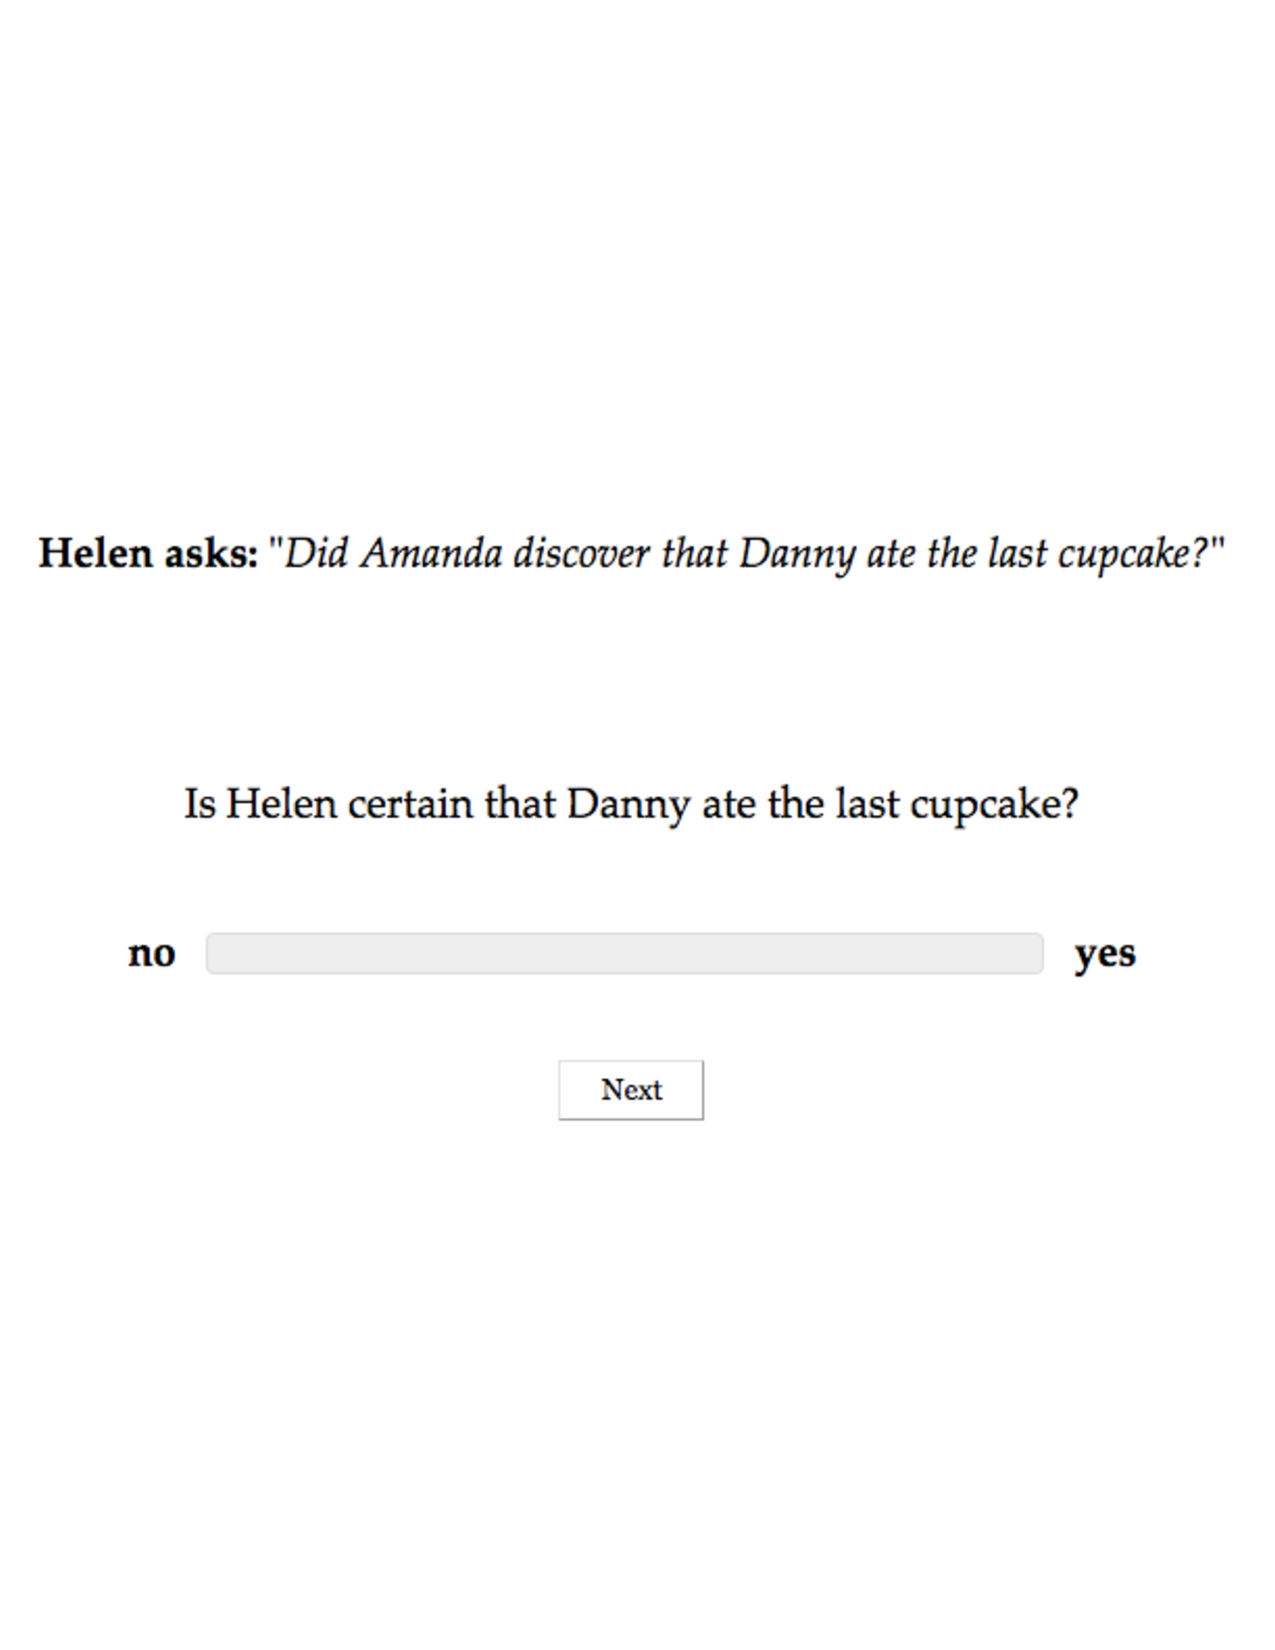
\includegraphics[width=10cm]{figures/trial-exp1}}
\end{center}
\caption{A sample trial in Experiment 1}\label{fig-trial-exp1}
\end{figure}

After completing the experiment, participants filled out a short, optional survey about their age, their gender, their native language(s) and, if English is their native language, whether they are a speaker of American English (as opposed to, e.g., Australian or Indian English). To encourage them to respond truthfully, participants were told that they would be paid no matter what answers they gave in the survey.


 
\section{Experiment}\label{s3}

The 20 sentences denoting the normed contents were realized as the complements of 20 clause-embedding predicates, for a total of 400 predicate/complement combinations. These combinations were realized as polar questions with a random subject noun phrase. In the target stimuli, the 400 polar questions were combined with one of the two facts that each content was normed with, for a total of 800 target stimuli. As shown in the sample target stimulus in (\ref{stim}), the named speaker (here, Carol) was explicitly stated to be aware of the fact.

\begin{figure}[h]
\centering
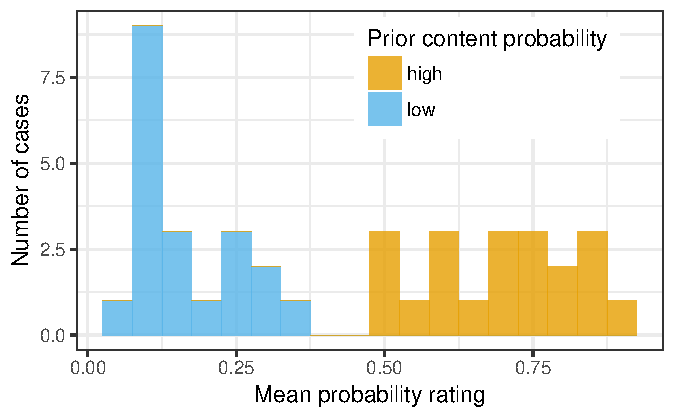
\includegraphics[width=.32\paperwidth]{../../results/1-prior/graphs/meanprobratings}
\caption{Histogram of mean prior probability ratings for each item (i.e., content/fact combination). Color indicates whether item was coded as high or low probability in the projectivity analysis.}\label{f-prior}
\end{figure}


\begin{exe}
\ex\label{stim}
{\bf Fact (which Carol knows):} Julian is German.  \\ 
{\bf Carol:} Does Sandra know that Julian dances salsa?
\end{exe}

The 20 predicates included the 5 factives {\em be annoyed, know, see, discover} and {\em reveal}, as well as 15 non-factives: the CC of 9 of these ({\em acknowledge, admit, announce, confess, confirm, establish, hear, inform, prove}) has been described as being able to project (e.g., \citealt{schlenker10,anand-hacquard2014,spector-egre2015,tbd-variability}), in contrast to that of the remaining 6 predicates ({\em pretend, suggest, say, think, be right, demonstrate}).



\noindent Projectivity was measured with the `certain that' diagnostic, following \citealt{tbd-variability}: for (\ref{stim}), participants judged whether Carol is certain that Julian dances salsa. Participants rated 20 target items (one for each predicate) and 6 control items (as attention checks). They responded on a sliding scale from `no' (no projection, coded 0) to `yes' (maximal projection, coded 1).

\begin{figure}[h]
\centering
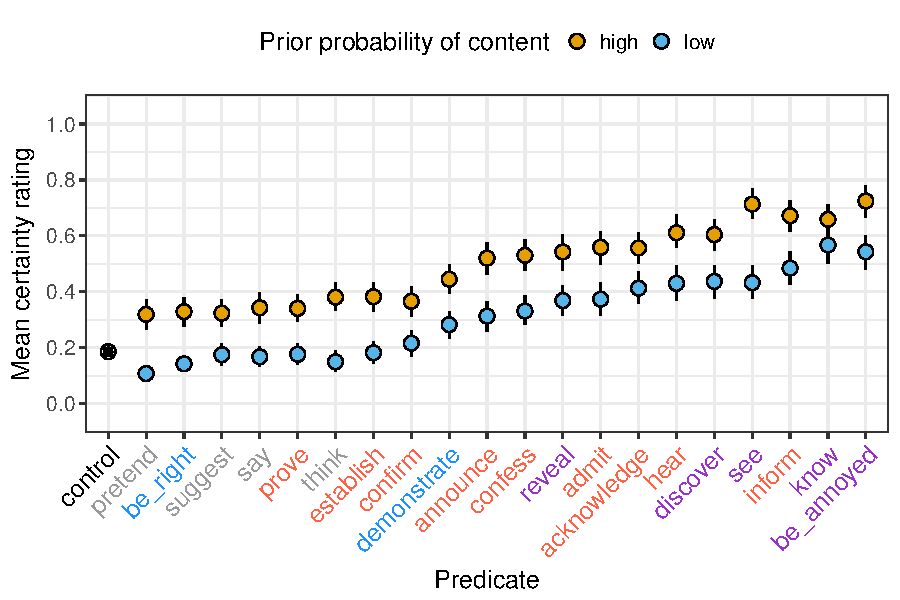
\includegraphics[width=.45\paperwidth]{../../results/3-projectivity/graphs/means-projectivity-by-predicate-and-facttype}
\caption{Mean certainty rating by predicate (x-axis) and prior CC probability, with 95\% CIs; factives in green.}\label{f-proj}
\end{figure}

\noindent
{\bf Results.} As shown in Fig.~\ref{f-proj}, mean certainty ratings for CCs were higher when the content had a higher prior probability than when it had a lower prior probability, as hypothesized by \citet{tbd-variability}. Furthermore, the effect of prior CC probability on projectivity was present across all 20 predicates, factive and non-factive ones. We also observe by-predicate variability in mean certainty ratings:  e.g., the means for factive {\em be annoyed} were higher, at .72 (high) / .53 (low), than those for factive {\em reveal}, at .55 / .37, which were higher than those for non-factive {\em establish}, at .39 / .19. These findings replicate \citetpos{tbd-variability} finding that projectivity is a gradient property of utterance content.

A linear mixed-effects model predicting certainty rating from prior probability (high vs.\ low) and verb (reference levels: low prior probability, {\em pretend}) with random intercepts for participant and item and a random by-participant slope for prior probability revealed a significant main effect of prior probability ($\beta$ = .19, SE = .01, t = 13.39, $p <$ .0001) and significantly higher certainty ratings for all predicates except for {\em be right} and {\em suggest} (5520 data points). A model that included an interaction term for the fixed effects was not significantly better than the model reported here.


\section{Discussion}

These results support \citetpos{tbd-variability} hypothesis that prior content probability influences projectivity. The finding that the CC of many non-factive predicates is at least weakly projective, even with low prior probability CCs, confirms intuitions reported in, e.g., \citealt{schlenker10}, \citealt{anand-hacquard2014} and \citealt{spector-egre2015}. These findings motivate the development of projection analyses that derive the influence of prior content probability and make predictions for the CCs of a broad range of both factive and non-factive predicates.

Current projection analyses, while limited to the CCs of factive predicates (e.g., \citealt{heim83,vds92,abrusan2011,brst-salt10,brst-ar}), are compatible with the finding that prior content probability influences projectivity. \citealt{heim83}, for instance, assumes default global accommodation when a presupposition is not entailed by the common ground (CG) when the trigger is uttered. This default is overridden when the presupposition is inconsistent with the CG. If we can assume that Julian dancing salsa is more likely to be consistent with the CG when Julian is from Cuba than when he is from Germany, \citealt{heim83} predicts that the presupposition that Julian dances salsa is more projective when it has a higher prior probability. 

As shown in Fig.~\ref{f-proj}, the CCs of several non-factives, including {\em inform, hear, acknowledge} and {\em admit}, are at least as projective as that of factive {\em reveal}. This finding challenges the long-standing assumption that the CCs of factives are more projective than those of non-factives. We suggest that this motivates constraint-based analyses that derive the projectivity of utterance content from the integration of multiple cues, including prior CC probability, the meanings of clause-embedding predicates, at-issueness (\citealt{tbd-variability}), and information structure (\citealt{tonhauser-salt26}).

\section{Conclusions}

\appendix

\setcounter{table}{0}
\renewcommand{\thetable}{A\arabic{table}}

\setcounter{figure}{0}
\renewcommand{\thefigure}{A\arabic{figure}}

\section{20 complement clauses}\label{a-clauses}

The following clauses realized the complements of the predicates in the experiment.

\begin{enumerate}[leftmargin=3ex,itemsep=-2pt]

\begin{multicols}{2}

\item Mary is pregnant.
\item Josie went on vacation to France.
\item Emma studied on Saturday morning.
\item Olivia sleeps until noon.
\item Sophia got a tattoo.
\item Mia drank 2 cocktails last night.
\item Isabella ate a steak on Sunday.
\item  Emily bought a car yesterday.
\item  Grace visited her sister.
\item Zoe calculated the tip.

\columnbreak

\item  Danny ate the last cupcake.
\item  Frank got a cat.
\item  Jackson ran 10 miles.
\item  Jayden rented a car.
\item  Tony had a drink last night.
\item  Josh learned to ride a bike yesterday.
\item  Owen shoveled snow last winter.
\item  Julian dances salsa.
\item  Jon walks to work.
\item  Charley speaks Spanish.

\end{multicols}

\end{enumerate}


\section{Initial experiments}\label{a-exp}

\subsection{Prior probability}

Prior probability was measured for 20 contents denoted by English sentences (e.g., Julian dances salsa) given a fact that made the content more likely (e.g., Julian is from Cuba) and a fact that made it less likely (e.g., Julian is from Germany). Participants were asked how likely a content is given a fact (e.g., Fact: Julian is from Cuba. How likely is it that Julian dances salsa?) and provided ratings on a sliding scale from `impossible' (interpreted as a probability of 0) to `definitely' (interpreted as a probability of 1). The mean ratings were .7 for high- and .16 for low-probability contents, see Fig.~\ref{f-prior} for the full set of items.

\paragraph{Participants}

\paragraph{Materials} The materials for the prior probability experiment consisted of...

\paragraph{Procedure}

\paragraph{Findings}

\subsection{Projection}

\paragraph{Participants} 300 participants with U.S.\ IP addresses and at least 99\% of previous HITs approved were recruited on Amazon's Mechanical Turk platform (ages: 20-71, median: 36; 136 female, 157 male, 2 other, 3 undeclared). They were paid 75 cents for participating in the experiment.

\paragraph{Materials} The materials for the projection experiment consisted of...

\paragraph{Procedure}

\paragraph{Data exclusion}
Prior to analysis, the data from 13 participants who did not self-identify as native speakers of American English were excluded. To assess whether the remaining 287 participants attended to the task, we inspected their responses to the 6 control stimuli, for which we expected low responses. We excluded the data from 16 participants whose response means on the controls were more than 2 standard deviations above the group mean. We furthermore identified 5 participants whose variance in overall response distribution was more than 2 standard deviations below the mean by-participant variance: these participants always selected roughly the same point on the response scale. We excluded the data from these 5 participants, too, leaving data from 266 participants (ages 20-71; median: 36; 118 female, 143 male, 2 other, 3 undeclared).

\paragraph{Findings}


\bibliographystyle{/Users/tonhauser.1/Library/Latex/cslipubs-natbib}
\bibliography{/Users/tonhauser.1/Documents/bibliography}

\end{document}

